\documentclass[10pt,a4paper]{article}

%double si on veut une version prof et une version élève. simple si on veut une seule version.
\newcommand{\buildmode}{double}

\InputIfFileExists{version.tex}{}{}
% Version (définie par le script)
\providecommand{\version}{eleve}

\usepackage{feuilleexo}

%%%à modifier à chaque fois

\renewcommand{\niveau}{2nde}
\renewcommand{\chapitre}{Équations, solution d'inéquations}
\renewcommand{\numchap}{0.3} 
\renewcommand{\theme}{Nombres et calcul}

\begin{document}

\prof{
    On a revu les notions de base semaine 1. L'objectif est d'être plus formel, et de marquer une trace dans le cours.
}
%\legendeicones

\vspace{-0.3cm}

\begin{prerequis}
\begin{itemize}
    \item Savoir calculer l'image d'une fonction.
    \item Être capable de remplir un tableau de valeurs
    \item Savoir lire et exploiter la représentation graphique d'une fonction.
\end{itemize}
\end{prerequis}

\begin{multicols}{2}

    \prof{
        Objectif : Formaliser la notion de fonctions. Avoir un vocabulaire plus précis afin que les prochains chapitres sur les fonctions soient plus clairs.
    }
\section{Calculs d'image et d'antécédents}
\begin{exo}[][]
    Quelle est l'image de 0 par la fonction \(f\) définie par \(f(x)=x^2-3x+4\) ; où \(x\) représente un nombre quelconque (dans l'intervalle \(]-\infty\ ;\ +\infty[\))
\end{exo}

\begin{exo}[][]
    Calculer \(g(3)\) sachant que \(g(x) = 2x-4\) pour tout nombre \(x\)
\end{exo}

\begin{exo}[][]
    Déterminer l'antécédent de 4 par la fonction \(h\) définie sur  \(]\infty\ ;\ +\infty[\) par \(h(x) = 2x+1\)
\end{exo}
\section{Tableau et ensemble de définition}

\begin{exo}
    Les vétérinaires donnent parfois le tableau de correspondance entre l'âge des chats et l'équivalent en âge humain ci-dessous.
    
    \begin{tabular}{|p{2cm}|*{6}{c|}}
        \hline
        Âge du chat (en années) & \(\dfrac{1}{2}\) & 1 & 2 & 6 & 12 & 16 \\ \hline
        Âge humain (en années) & 10 & 18 & 26 & 42 & 70 & 94 \\ \hline
    \end{tabular}

    On note \(c\) l'âge du chat en années et \(H(c)\) l'âge humain équivalent années.
    \begin{enumerate}
        \item Dans le repère ci-dessous, tracer une courbe représentant la fonction \(H\) sur l'intervalle \([0;\ \ 16]\).
        
        \hspace{-1.5cm}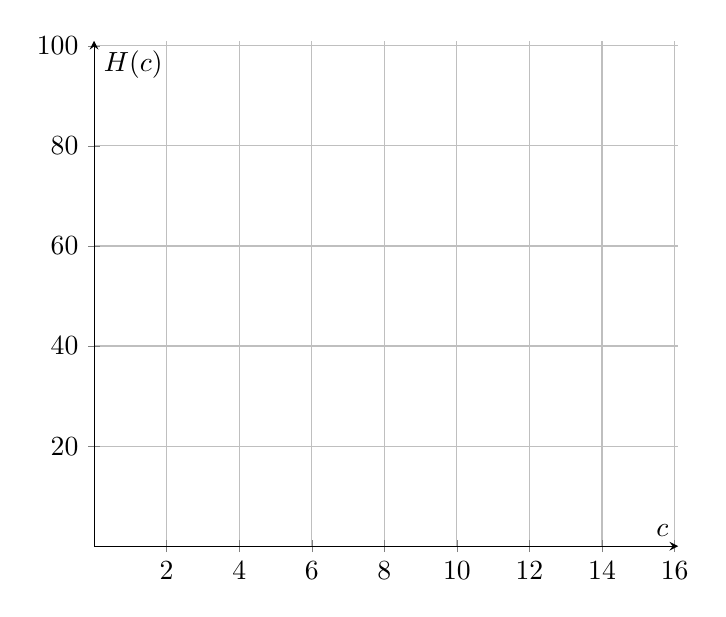
\begin{tikzpicture}
        \begin{axis}[
            axis lines=middle,
            xmin=-0, xmax=16.1,
            ymin=0, ymax=101,
            domain=-2:2,
            samples=300,
            grid=major,
            xtick={0,2,...,16},
            ytick={0,20,...,100},
            xlabel={\(c\)},
            ylabel={\(H(c)\)},
            width=9cm,
            height=8cm
        ]

        \end{axis}
        \end{tikzpicture}
        \item Les deux âges sont-ils proportionnels ? Justifier.
        \item Préciser l'image de 3 et interpréter la réponse.
        \item Donner un antécédent de 60 et interpréter la réponse.
    \end{enumerate}
\end{exo}

\begin{exo}[QCM][]
    
    \begin{tabular}{|*{5}{c|}}
        \hline
        \(t\) & 2 & 3 & 4 & 5 \\
        \hline
        \(k(t)\) & 5 & 10 & 17 & 26 \\
        \hline
    \end{tabular}

    Avec la table de valeur ci-dessus, \(k(t)\) peut être égal à \begin{tasks}(4)
    \task \(2t+1\)
    \task \(3t+1\)
    \task \(t^2-1\)
    \task \(t^2+1\)
    \end{tasks}
\end{exo}

\begin{exo}[][appro]
    On considère la fonction \(f\) définie par \(f(x) = \dfrac{x}{2x-2}\)
    \begin{enumerate}
        \item Remplir le tableau de valeur ci-dessous
    
        \renewcommand{\arraystretch}{2}
    \begin{tabular}{|*{7}{c|}}
        \hline
        \(x\) & \(-1\) & \(0\) & \(\dfrac{1}{2}\) & \(1\) & \(\dfrac{3}{2}\) & \(3\)  \\
        \hline
        \(f(x)\) & & & & & & \\
        \hline
    \end{tabular}

    \item Existe-t-il un nombre qui n'a pas d'image ? Si oui, comment l'expliquer ?
    \item Comment pourrait-on écrire l'ensemble de définition de \(f\) ?
    \end{enumerate}

    \prof{
        Dernière question pas necessaire si on s'en ressert pas
    }
\end{exo}

\begin{exo}[][avance]
    On considère la fonction \(g\) définie par \(g(x) = \dfrac{1}{x^2-9}\)
    \begin{enumerate}
        \item Remplir le tableau de valeur ci-dessous.
    
        \renewcommand{\arraystretch}{2}
    \begin{tabular}{|*{7}{c|}}
        \hline
        \(x\) & \(-3\) & \(-1\) & \(0\) & \(1\) & 2 & \(3\)  \\
        \hline
        \(g(x)\) & & & & & & \\
        \hline
    \end{tabular}

    \item Quel est l'ensemble de définition de \(g\) ?
    \item Comment pourrait-on le démontrer ?
    \end{enumerate}
\end{exo}

\section{Représentation graphique}

\begin{exo}[][]
    On considère une fonction \(f\) dont la représentation graphique est donnée ci-dessous.

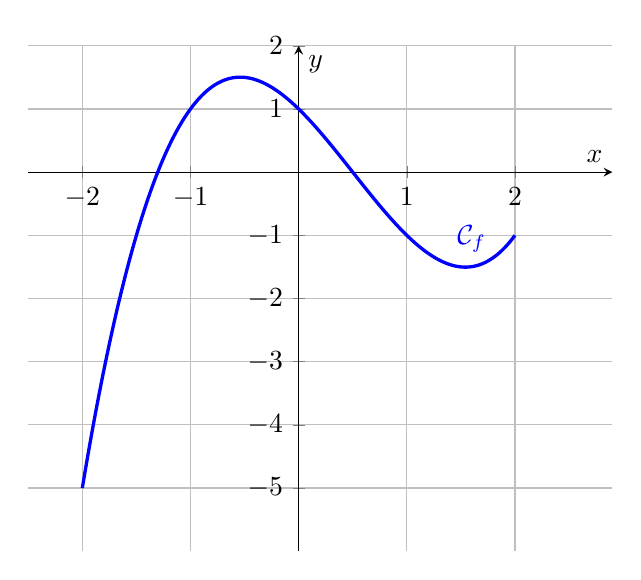
\begin{tikzpicture}
\begin{axis}[
    axis lines=middle,
    xmin=-2.5, xmax=2.9,
    ymin=-6, ymax=2,
    domain=-2:2,
    samples=300,
    grid=major,
    xtick={-2,-1,0,1,2,3},
    ytick={-5,-4,-3,-2,-1,0,1,2,3,4},
    xlabel={\(x\)},
    ylabel={\(y\)},
    width=9cm,
    height=8cm
]

\addplot[
    blue,
    very thick
] {2/3*(x-2)*(x+1.5)*(x-1)-1}
node[pos=0.92, above right] {\(\mathcal{C}_f\)};

\end{axis}
\end{tikzpicture}

\begin{enumerate}[leftmargin=*]
    \item Quel est l'ensemble de définition de \(f\) ?
    \item Donner les images de \(-2\), \(0\) et \(1\) par \(f\).
    \item Donner les éventuels antécédents de -1 et de 1.
    \item Résoudre \(f(x)=0\).
\end{enumerate}
\end{exo}

\begin{exo}[Vrai ou faux][appro]
    \begin{enumerate}
        \item Un nombre peut avoir deux images différentes par la même fonction.
        \item Un nombre peut avoir zéro, un, ou plusieurs antécédents par une fonction.
        \medbreak
        On considère la fonction \(h\) définie sur l'intervalle [-5\ ;\ 5] dont la représentation graphique est la suivante :

        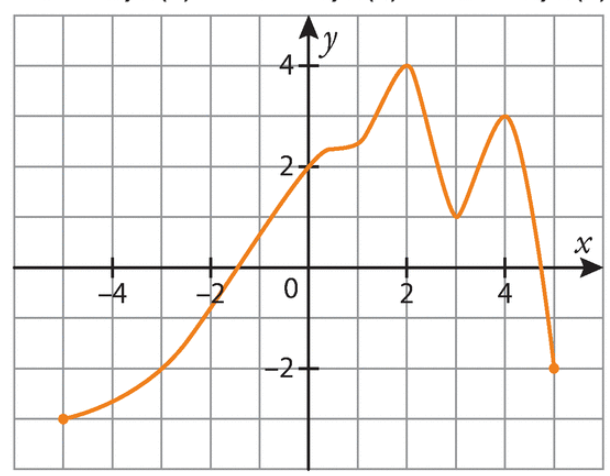
\includegraphics[width=0.4\textwidth]{fonction1.png}

        \item Le nombre \(6\) a une image par \(h\)
        \item Le nombre 0 a plusieurs antécédents par \(h\).
    \end{enumerate}
\end{exo}

\begin{exo}[][appro]
\(f\) est définie sur \([-2 ; 2]\) dont on donne le tableau de valeurs suivant :

\renewcommand{\arraystretch}{2.5}
\begin{tabular}{|*{10}{c|}}
    \hline
    \(x\) & \(-2\)& \(-\dfrac{3}{2}\)& \(-1\)& \(-\dfrac{1}{2}\)& \(0\)& \(\dfrac{1}{2}\)& \(1\) & \(\dfrac{3}{2}\) & \(2\) \\ \hline
    \(f(x)\) & \(-1\) & \(-3\) & \(-1\) & \(3\) & \(2\) &  \(0\) &  \(2\) & \(1\) &   \(3\) \\ \hline
\end{tabular}

\medbreak
Quatre élèves proposent une représentation graphique de \(f\). \\

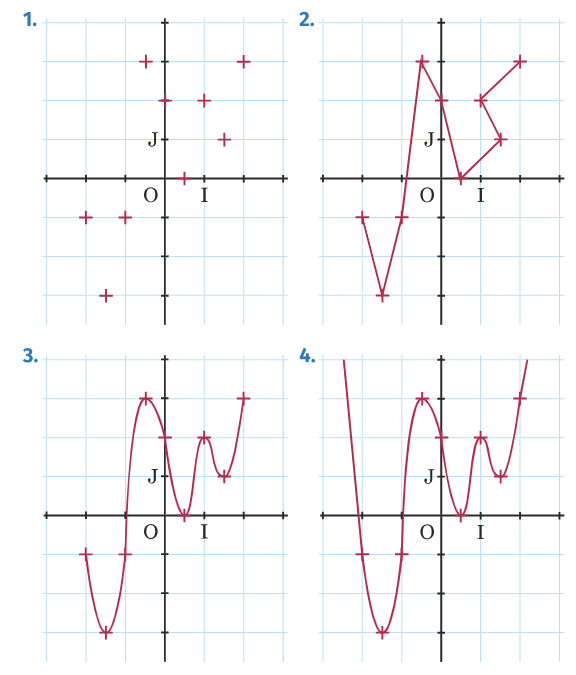
\includegraphics[width=0.4\textwidth]{quatre_fonctions.png}

Laquelle de ces courbes vous semblent le plus satisfaisantes ? Justifier.
\end{exo}

\begin{exo}[Avec calculatrice][]
    On considère un cône ayant un diamètre \(x\) égal à sa hauteur.

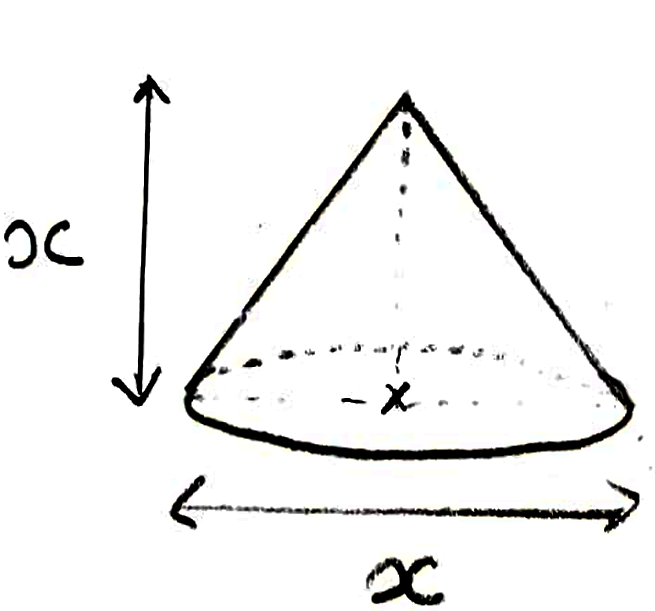
\includegraphics[width=0.2\textwidth]{cone.png}

    Son volume s'obtient par la formule \[ V(x) = \dfrac{1}{6}\pi x^3 \]. Sur le graphique, on a représenté graphiquement la fonction \(V\) pour \(x\) dans l'interrvalle \([0\ ;\ 8]\).

    \medbreak
    \textit{Indiquer à l'aide de pointillés chaque lecture graphique.}
    \begin{enumerate}
        \item Par lecture graphique, donner une valeur approchée du nombre \(V(6)\).
        \item Calculer la valeur exacte de \(V(6)\)
        \item En déduire une valeur arrondie à l'unité de l'image du nombre \(6\) par la fonction \(V\).
        \item Par lecture graphique, donner une valeur approchée de l'antécédent du nombre 200 par la fonction \(V\).
    \end{enumerate}

    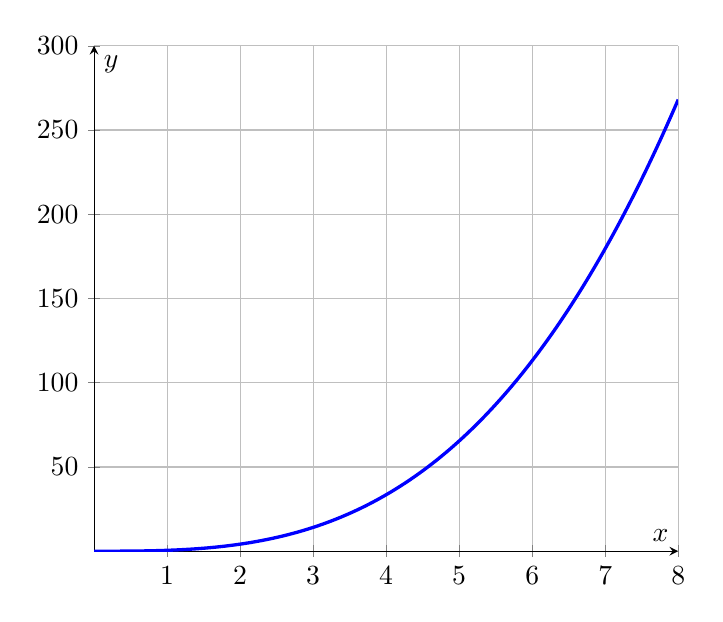
\begin{tikzpicture}
    \begin{axis}[
        axis lines=middle,
        xmin=0, xmax=8,
        ymin=0, ymax=300,
        domain=0:8,
        samples=300,
        grid=major,
        xtick={0,1,...,8},
        ytick={0,50,...,300},
        xlabel={\(x\)},
        ylabel={\(y\)},
        width=9cm,
        height=8cm
    ]

    \addplot[
        blue,
        very thick
    ] {1/6*pi*x^3};
    \end{axis}
    \end{tikzpicture}
\end{exo}
\end{multicols}

\end{document}
